% Options for packages loaded elsewhere
\PassOptionsToPackage{unicode}{hyperref}
\PassOptionsToPackage{hyphens}{url}
%
\documentclass[
]{article}
\usepackage{amsmath,amssymb}
\usepackage{iftex}
\ifPDFTeX
  \usepackage[T1]{fontenc}
  \usepackage[utf8]{inputenc}
  \usepackage{textcomp} % provide euro and other symbols
\else % if luatex or xetex
  \usepackage{unicode-math} % this also loads fontspec
  \defaultfontfeatures{Scale=MatchLowercase}
  \defaultfontfeatures[\rmfamily]{Ligatures=TeX,Scale=1}
\fi
\usepackage{lmodern}
\ifPDFTeX\else
  % xetex/luatex font selection
\fi
% Use upquote if available, for straight quotes in verbatim environments
\IfFileExists{upquote.sty}{\usepackage{upquote}}{}
\IfFileExists{microtype.sty}{% use microtype if available
  \usepackage[]{microtype}
  \UseMicrotypeSet[protrusion]{basicmath} % disable protrusion for tt fonts
}{}
\makeatletter
\@ifundefined{KOMAClassName}{% if non-KOMA class
  \IfFileExists{parskip.sty}{%
    \usepackage{parskip}
  }{% else
    \setlength{\parindent}{0pt}
    \setlength{\parskip}{6pt plus 2pt minus 1pt}}
}{% if KOMA class
  \KOMAoptions{parskip=half}}
\makeatother
\usepackage{xcolor}
\usepackage[margin=1in]{geometry}
\usepackage{color}
\usepackage{fancyvrb}
\newcommand{\VerbBar}{|}
\newcommand{\VERB}{\Verb[commandchars=\\\{\}]}
\DefineVerbatimEnvironment{Highlighting}{Verbatim}{commandchars=\\\{\}}
% Add ',fontsize=\small' for more characters per line
\usepackage{framed}
\definecolor{shadecolor}{RGB}{248,248,248}
\newenvironment{Shaded}{\begin{snugshade}}{\end{snugshade}}
\newcommand{\AlertTok}[1]{\textcolor[rgb]{0.94,0.16,0.16}{#1}}
\newcommand{\AnnotationTok}[1]{\textcolor[rgb]{0.56,0.35,0.01}{\textbf{\textit{#1}}}}
\newcommand{\AttributeTok}[1]{\textcolor[rgb]{0.13,0.29,0.53}{#1}}
\newcommand{\BaseNTok}[1]{\textcolor[rgb]{0.00,0.00,0.81}{#1}}
\newcommand{\BuiltInTok}[1]{#1}
\newcommand{\CharTok}[1]{\textcolor[rgb]{0.31,0.60,0.02}{#1}}
\newcommand{\CommentTok}[1]{\textcolor[rgb]{0.56,0.35,0.01}{\textit{#1}}}
\newcommand{\CommentVarTok}[1]{\textcolor[rgb]{0.56,0.35,0.01}{\textbf{\textit{#1}}}}
\newcommand{\ConstantTok}[1]{\textcolor[rgb]{0.56,0.35,0.01}{#1}}
\newcommand{\ControlFlowTok}[1]{\textcolor[rgb]{0.13,0.29,0.53}{\textbf{#1}}}
\newcommand{\DataTypeTok}[1]{\textcolor[rgb]{0.13,0.29,0.53}{#1}}
\newcommand{\DecValTok}[1]{\textcolor[rgb]{0.00,0.00,0.81}{#1}}
\newcommand{\DocumentationTok}[1]{\textcolor[rgb]{0.56,0.35,0.01}{\textbf{\textit{#1}}}}
\newcommand{\ErrorTok}[1]{\textcolor[rgb]{0.64,0.00,0.00}{\textbf{#1}}}
\newcommand{\ExtensionTok}[1]{#1}
\newcommand{\FloatTok}[1]{\textcolor[rgb]{0.00,0.00,0.81}{#1}}
\newcommand{\FunctionTok}[1]{\textcolor[rgb]{0.13,0.29,0.53}{\textbf{#1}}}
\newcommand{\ImportTok}[1]{#1}
\newcommand{\InformationTok}[1]{\textcolor[rgb]{0.56,0.35,0.01}{\textbf{\textit{#1}}}}
\newcommand{\KeywordTok}[1]{\textcolor[rgb]{0.13,0.29,0.53}{\textbf{#1}}}
\newcommand{\NormalTok}[1]{#1}
\newcommand{\OperatorTok}[1]{\textcolor[rgb]{0.81,0.36,0.00}{\textbf{#1}}}
\newcommand{\OtherTok}[1]{\textcolor[rgb]{0.56,0.35,0.01}{#1}}
\newcommand{\PreprocessorTok}[1]{\textcolor[rgb]{0.56,0.35,0.01}{\textit{#1}}}
\newcommand{\RegionMarkerTok}[1]{#1}
\newcommand{\SpecialCharTok}[1]{\textcolor[rgb]{0.81,0.36,0.00}{\textbf{#1}}}
\newcommand{\SpecialStringTok}[1]{\textcolor[rgb]{0.31,0.60,0.02}{#1}}
\newcommand{\StringTok}[1]{\textcolor[rgb]{0.31,0.60,0.02}{#1}}
\newcommand{\VariableTok}[1]{\textcolor[rgb]{0.00,0.00,0.00}{#1}}
\newcommand{\VerbatimStringTok}[1]{\textcolor[rgb]{0.31,0.60,0.02}{#1}}
\newcommand{\WarningTok}[1]{\textcolor[rgb]{0.56,0.35,0.01}{\textbf{\textit{#1}}}}
\usepackage{graphicx}
\makeatletter
\def\maxwidth{\ifdim\Gin@nat@width>\linewidth\linewidth\else\Gin@nat@width\fi}
\def\maxheight{\ifdim\Gin@nat@height>\textheight\textheight\else\Gin@nat@height\fi}
\makeatother
% Scale images if necessary, so that they will not overflow the page
% margins by default, and it is still possible to overwrite the defaults
% using explicit options in \includegraphics[width, height, ...]{}
\setkeys{Gin}{width=\maxwidth,height=\maxheight,keepaspectratio}
% Set default figure placement to htbp
\makeatletter
\def\fps@figure{htbp}
\makeatother
\setlength{\emergencystretch}{3em} % prevent overfull lines
\providecommand{\tightlist}{%
  \setlength{\itemsep}{0pt}\setlength{\parskip}{0pt}}
\setcounter{secnumdepth}{-\maxdimen} % remove section numbering
\ifLuaTeX
  \usepackage{selnolig}  % disable illegal ligatures
\fi
\usepackage{bookmark}
\IfFileExists{xurl.sty}{\usepackage{xurl}}{} % add URL line breaks if available
\urlstyle{same}
\hypersetup{
  pdftitle={Goodplot/Badplot},
  pdfauthor={Jobel Y. Villafane Pagan},
  hidelinks,
  pdfcreator={LaTeX via pandoc}}

\title{Goodplot/Badplot}
\author{Jobel Y. Villafane Pagan}
\date{2024-10-26}

\begin{document}
\maketitle

\#Introduction The homework is to creating two version of similar plots,
using Taylor Swift data. Welcome to the bad plot/good plot!

\begin{figure}
\centering
\includegraphics{https://preview.redd.it/every-artist-has-taylors-version-v0-6igip3ycs57c1.jpeg?auto=webp&s=b1f7507aae766f7b0248918719af40d5e1c590bc}
\caption{Taylor}
\end{figure}

\#Load libraries

\begin{Shaded}
\begin{Highlighting}[]
\FunctionTok{library}\NormalTok{(tidyverse)}
\FunctionTok{library}\NormalTok{(tidytuesdayR)}
\FunctionTok{library}\NormalTok{(here)}
\FunctionTok{library}\NormalTok{(taylor)}
\FunctionTok{library}\NormalTok{(ggplot2)}
\FunctionTok{library}\NormalTok{(dplyr)}
\FunctionTok{library}\NormalTok{(tayloRswift)}
\FunctionTok{library}\NormalTok{(gganimate)}
\end{Highlighting}
\end{Shaded}

\section{Inspect the data}\label{inspect-the-data}

\begin{Shaded}
\begin{Highlighting}[]
\NormalTok{tuesdata }\OtherTok{\textless{}{-}}\NormalTok{ tidytuesdayR}\SpecialCharTok{::}\FunctionTok{tt\_load}\NormalTok{(}\DecValTok{2023}\NormalTok{, }\AttributeTok{week =} \DecValTok{42}\NormalTok{)}

\NormalTok{taylor\_album\_songs }\OtherTok{\textless{}{-}}\NormalTok{ tuesdata}\SpecialCharTok{$}\NormalTok{taylor\_album\_songs}
\NormalTok{taylor\_all\_songs }\OtherTok{\textless{}{-}}\NormalTok{ tuesdata}\SpecialCharTok{$}\NormalTok{taylor\_all\_songs}
\NormalTok{taylor\_albums }\OtherTok{\textless{}{-}}\NormalTok{ tuesdata}\SpecialCharTok{$}\NormalTok{taylor\_albums}

\FunctionTok{glimpse}\NormalTok{(taylor\_album\_songs)}
\end{Highlighting}
\end{Shaded}

\begin{verbatim}
## Rows: 194
## Columns: 29
## $ album_name          <chr> "Taylor Swift", "Taylor Swift", "Taylor Swift", "T~
## $ ep                  <lgl> FALSE, FALSE, FALSE, FALSE, FALSE, FALSE, FALSE, F~
## $ album_release       <date> 2006-10-24, 2006-10-24, 2006-10-24, 2006-10-24, 2~
## $ track_number        <dbl> 1, 2, 3, 4, 5, 6, 7, 8, 9, 10, 11, 12, 13, 14, 15,~
## $ track_name          <chr> "Tim McGraw", "Picture To Burn", "Teardrops On My ~
## $ artist              <chr> "Taylor Swift", "Taylor Swift", "Taylor Swift", "T~
## $ featuring           <chr> NA, NA, NA, NA, NA, NA, NA, NA, NA, NA, NA, NA, NA~
## $ bonus_track         <lgl> FALSE, FALSE, FALSE, FALSE, FALSE, FALSE, FALSE, F~
## $ promotional_release <date> NA, NA, NA, NA, NA, NA, NA, NA, NA, NA, NA, NA, N~
## $ single_release      <date> 2006-06-19, 2008-02-03, 2007-02-19, NA, NA, NA, N~
## $ track_release       <date> 2006-06-19, 2006-10-24, 2006-10-24, 2006-10-24, 2~
## $ danceability        <dbl> 0.580, 0.658, 0.621, 0.576, 0.418, 0.589, 0.479, 0~
## $ energy              <dbl> 0.491, 0.877, 0.417, 0.777, 0.482, 0.805, 0.578, 0~
## $ key                 <dbl> 0, 7, 10, 9, 5, 5, 2, 8, 4, 2, 2, 8, 7, 4, 10, 5, ~
## $ loudness            <dbl> -6.462, -2.098, -6.941, -2.881, -5.769, -4.055, -4~
## $ mode                <dbl> 1, 1, 1, 1, 1, 1, 1, 1, 0, 1, 1, 1, 1, 1, 1, 1, 1,~
## $ speechiness         <dbl> 0.0251, 0.0323, 0.0231, 0.0324, 0.0266, 0.0293, 0.~
## $ acousticness        <dbl> 0.57500, 0.17300, 0.28800, 0.05100, 0.21700, 0.004~
## $ instrumentalness    <dbl> 0.00e+00, 0.00e+00, 0.00e+00, 0.00e+00, 0.00e+00, ~
## $ liveness            <dbl> 0.1210, 0.0962, 0.1190, 0.3200, 0.1230, 0.2400, 0.~
## $ valence             <dbl> 0.425, 0.821, 0.289, 0.428, 0.261, 0.591, 0.192, 0~
## $ tempo               <dbl> 76.009, 105.586, 99.953, 115.028, 175.558, 112.982~
## $ time_signature      <dbl> 4, 4, 4, 4, 4, 4, 4, 4, 4, 4, 4, 4, 4, 4, 4, 4, 4,~
## $ duration_ms         <dbl> 232107, 173067, 203040, 199200, 239013, 207107, 24~
## $ explicit            <lgl> FALSE, FALSE, FALSE, FALSE, FALSE, FALSE, FALSE, F~
## $ key_name            <chr> "C", "G", "A#", "A", "F", "F", "D", "G#", "E", "D"~
## $ mode_name           <chr> "major", "major", "major", "major", "major", "majo~
## $ key_mode            <chr> "C major", "G major", "A# major", "A major", "F ma~
## $ lyrics              <lgl> NA, NA, NA, NA, NA, NA, NA, NA, NA, NA, NA, NA, NA~
\end{verbatim}

\begin{Shaded}
\begin{Highlighting}[]
\FunctionTok{glimpse}\NormalTok{(taylor\_all\_songs)}
\end{Highlighting}
\end{Shaded}

\begin{verbatim}
## Rows: 274
## Columns: 29
## $ album_name          <chr> "Taylor Swift", "Taylor Swift", "Taylor Swift", "T~
## $ ep                  <lgl> FALSE, FALSE, FALSE, FALSE, FALSE, FALSE, FALSE, F~
## $ album_release       <date> 2006-10-24, 2006-10-24, 2006-10-24, 2006-10-24, 2~
## $ track_number        <dbl> 1, 2, 3, 4, 5, 6, 7, 8, 9, 10, 11, 12, 13, 14, 15,~
## $ track_name          <chr> "Tim McGraw", "Picture To Burn", "Teardrops On My ~
## $ artist              <chr> "Taylor Swift", "Taylor Swift", "Taylor Swift", "T~
## $ featuring           <chr> NA, NA, NA, NA, NA, NA, NA, NA, NA, NA, NA, NA, NA~
## $ bonus_track         <lgl> FALSE, FALSE, FALSE, FALSE, FALSE, FALSE, FALSE, F~
## $ promotional_release <date> NA, NA, NA, NA, NA, NA, NA, NA, NA, NA, NA, NA, N~
## $ single_release      <date> 2006-06-19, 2008-02-03, 2007-02-19, NA, NA, NA, N~
## $ track_release       <date> 2006-06-19, 2006-10-24, 2006-10-24, 2006-10-24, 2~
## $ danceability        <dbl> 0.580, 0.658, 0.621, 0.576, 0.418, 0.589, 0.479, 0~
## $ energy              <dbl> 0.491, 0.877, 0.417, 0.777, 0.482, 0.805, 0.578, 0~
## $ key                 <dbl> 0, 7, 10, 9, 5, 5, 2, 8, 4, 2, 2, 8, 7, 4, 10, 5, ~
## $ loudness            <dbl> -6.462, -2.098, -6.941, -2.881, -5.769, -4.055, -4~
## $ mode                <dbl> 1, 1, 1, 1, 1, 1, 1, 1, 0, 1, 1, 1, 1, 1, 1, 1, 1,~
## $ speechiness         <dbl> 0.0251, 0.0323, 0.0231, 0.0324, 0.0266, 0.0293, 0.~
## $ acousticness        <dbl> 0.57500, 0.17300, 0.28800, 0.05100, 0.21700, 0.004~
## $ instrumentalness    <dbl> 0.00e+00, 0.00e+00, 0.00e+00, 0.00e+00, 0.00e+00, ~
## $ liveness            <dbl> 0.1210, 0.0962, 0.1190, 0.3200, 0.1230, 0.2400, 0.~
## $ valence             <dbl> 0.425, 0.821, 0.289, 0.428, 0.261, 0.591, 0.192, 0~
## $ tempo               <dbl> 76.009, 105.586, 99.953, 115.028, 175.558, 112.982~
## $ time_signature      <dbl> 4, 4, 4, 4, 4, 4, 4, 4, 4, 4, 4, 4, 4, 4, 4, 4, 4,~
## $ duration_ms         <dbl> 232107, 173067, 203040, 199200, 239013, 207107, 24~
## $ explicit            <lgl> FALSE, FALSE, FALSE, FALSE, FALSE, FALSE, FALSE, F~
## $ key_name            <chr> "C", "G", "A#", "A", "F", "F", "D", "G#", "E", "D"~
## $ mode_name           <chr> "major", "major", "major", "major", "major", "majo~
## $ key_mode            <chr> "C major", "G major", "A# major", "A major", "F ma~
## $ lyrics              <lgl> NA, NA, NA, NA, NA, NA, NA, NA, NA, NA, NA, NA, NA~
\end{verbatim}

\begin{Shaded}
\begin{Highlighting}[]
\FunctionTok{glimpse}\NormalTok{(taylor\_albums)}
\end{Highlighting}
\end{Shaded}

\begin{verbatim}
## Rows: 14
## Columns: 5
## $ album_name       <chr> "Taylor Swift", "The Taylor Swift Holiday Collection"~
## $ ep               <lgl> FALSE, TRUE, TRUE, FALSE, FALSE, FALSE, FALSE, FALSE,~
## $ album_release    <date> 2006-10-24, 2007-10-14, 2008-07-15, 2008-11-11, 2010~
## $ metacritic_score <dbl> 67, NA, NA, 73, 77, 77, 76, 71, 79, 88, 85, 82, 91, 85
## $ user_score       <dbl> 8.5, NA, NA, 8.4, 8.6, 8.5, 8.2, 8.3, 8.4, 9.0, 8.9, ~
\end{verbatim}

\begin{Shaded}
\begin{Highlighting}[]
\FunctionTok{view}\NormalTok{(taylor\_album\_songs)}
\FunctionTok{view}\NormalTok{(taylor\_all\_songs)}
\FunctionTok{view}\NormalTok{(taylor\_albums)}
\end{Highlighting}
\end{Shaded}

\begin{Shaded}
\begin{Highlighting}[]
\CommentTok{\# scatter plot of Metacritic Score by Album Release Date}
\FunctionTok{ggplot}\NormalTok{(taylor\_albums, }\FunctionTok{aes}\NormalTok{(}\AttributeTok{x =}\NormalTok{ album\_release, }
                          \AttributeTok{y =}\NormalTok{ metacritic\_score, }
                          \AttributeTok{color =}\NormalTok{ album\_name)) }\SpecialCharTok{+} 
  \FunctionTok{geom\_point}\NormalTok{(}\AttributeTok{size =} \DecValTok{5}\NormalTok{) }\SpecialCharTok{+}  
  \FunctionTok{geom\_line}\NormalTok{(}\FunctionTok{aes}\NormalTok{(}\AttributeTok{group =}\NormalTok{ album\_name), }\AttributeTok{size =} \DecValTok{2}\NormalTok{) }\SpecialCharTok{+}  \CommentTok{\# Connect points with a trend line}
  \FunctionTok{geom\_smooth}\NormalTok{(}\AttributeTok{method =} \StringTok{"loess"}\NormalTok{, }\AttributeTok{se =} \ConstantTok{FALSE}\NormalTok{, }\AttributeTok{color =} \StringTok{"black"}\NormalTok{, }\AttributeTok{linetype =} \StringTok{"dashed"}\NormalTok{) }\SpecialCharTok{+}
  \FunctionTok{geom\_text}\NormalTok{(}\FunctionTok{aes}\NormalTok{(}\AttributeTok{label =}\NormalTok{ album\_name), }\AttributeTok{vjust =} \SpecialCharTok{{-}}\DecValTok{1}\NormalTok{, }\AttributeTok{size =} \DecValTok{3}\NormalTok{, }\AttributeTok{face =} \StringTok{"bold"}\NormalTok{) }\SpecialCharTok{+}  \CommentTok{\# Add album names as labels above points}
  \FunctionTok{labs}\NormalTok{(}\AttributeTok{title =} \StringTok{"Taylor Swift Discography Evolution"}\NormalTok{,}
       \AttributeTok{subtitle =}  \StringTok{"Metacritic given score by musical album relased (2006 to 2022)"}\NormalTok{,}
       \AttributeTok{x =} \StringTok{"Album Release Date"}\NormalTok{,}
       \AttributeTok{y =} \StringTok{"Metacritic Score"}\NormalTok{) }\SpecialCharTok{+}
  
  \FunctionTok{scale\_color\_taylor}\NormalTok{(}\AttributeTok{palette =} \StringTok{"taylorRed"}\NormalTok{) }\SpecialCharTok{+}  \CommentTok{\# Apply Taylor\textquotesingle{}s color palette}
  \FunctionTok{theme\_minimal}\NormalTok{() }\SpecialCharTok{+}  \CommentTok{\# Minimal theme for a clean look}
  \FunctionTok{theme}\NormalTok{(}\AttributeTok{plot.title =} \FunctionTok{element\_text}\NormalTok{(}\AttributeTok{hjust =} \FloatTok{0.75}\NormalTok{, }\AttributeTok{face =} \StringTok{"bold"}\NormalTok{),  }\CommentTok{\# Center and bold the title}
        \AttributeTok{axis.text.x =} \FunctionTok{element\_text}\NormalTok{(}\AttributeTok{angle =} \DecValTok{45}\NormalTok{, }\AttributeTok{hjust =} \DecValTok{1}\NormalTok{),}
        \AttributeTok{legend.position =} \StringTok{"none"}\NormalTok{) }\SpecialCharTok{+}  \CommentTok{\# Remove the legend }
         \FunctionTok{ylim}\NormalTok{(}\DecValTok{65}\NormalTok{, }\DecValTok{95}\NormalTok{) }
\end{Highlighting}
\end{Shaded}

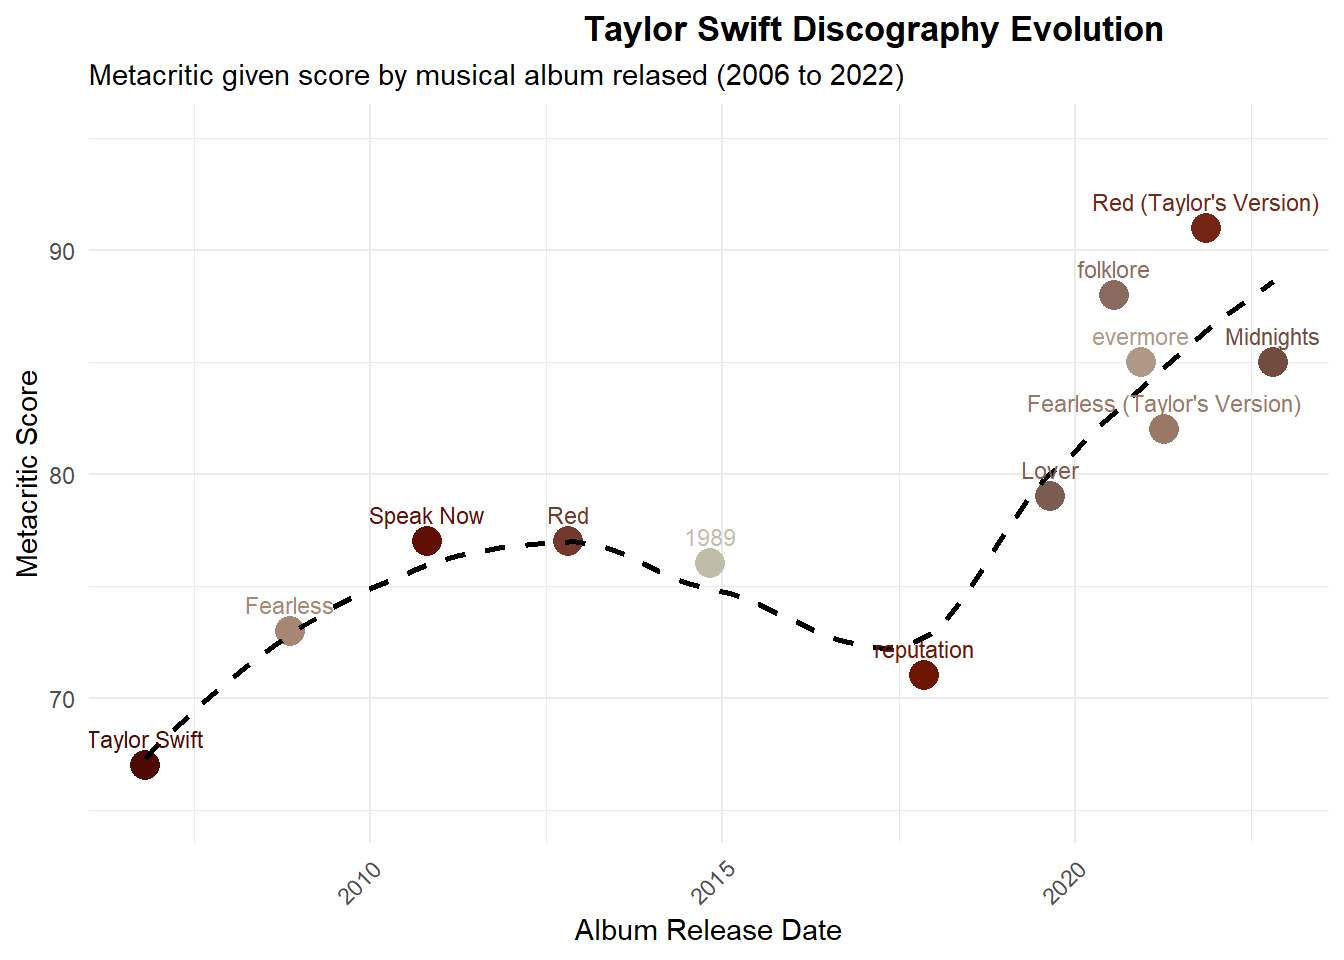
\includegraphics{../Output/unnamed-chunk-3-1.pdf}

\#Bad plot The plot represent a bad plot, due to several variables show
at the same time.

-Ugly -Multiple legends; one on the side (album\_name) and labels
(album\_name and \%) -the data is shown on a pie chart -the labels can't
be seeing, the chart is space inefficient -the chart can't be understand

\begin{Shaded}
\begin{Highlighting}[]
\CommentTok{\# Prepare data for the pie chart}
\NormalTok{pie\_data }\OtherTok{\textless{}{-}}\NormalTok{ taylor\_albums }\SpecialCharTok{\%\textgreater{}\%}
  \FunctionTok{group\_by}\NormalTok{(album\_name) }\SpecialCharTok{\%\textgreater{}\%}
  \FunctionTok{summarise}\NormalTok{(}\AttributeTok{total\_score =} \FunctionTok{sum}\NormalTok{(metacritic\_score, }\AttributeTok{na.rm =} \ConstantTok{TRUE}\NormalTok{)) }\SpecialCharTok{\%\textgreater{}\%}
  \FunctionTok{mutate}\NormalTok{(}\AttributeTok{percentage =}\NormalTok{ total\_score }\SpecialCharTok{/} \FunctionTok{sum}\NormalTok{(total\_score) }\SpecialCharTok{*} \DecValTok{100}\NormalTok{) }\SpecialCharTok{\%\textgreater{}\%}
  \FunctionTok{mutate}\NormalTok{(}\AttributeTok{label =} \FunctionTok{paste}\NormalTok{(album\_name, }\FunctionTok{round}\NormalTok{(percentage, }\DecValTok{1}\NormalTok{), }\StringTok{"\%"}\NormalTok{, }\AttributeTok{sep =} \StringTok{" "}\NormalTok{))}

\CommentTok{\# Create the pie chart}
\FunctionTok{ggplot}\NormalTok{(pie\_data, }\FunctionTok{aes}\NormalTok{(}\AttributeTok{x =} \StringTok{""}\NormalTok{, }
                     \AttributeTok{y =}\NormalTok{ percentage, }
                     \AttributeTok{fill =}\NormalTok{ album\_name)) }\SpecialCharTok{+}
  \FunctionTok{geom\_bar}\NormalTok{(}\AttributeTok{stat =} \StringTok{"identity"}\NormalTok{, }\AttributeTok{width =} \DecValTok{5}\NormalTok{) }\SpecialCharTok{+}
  \FunctionTok{coord\_polar}\NormalTok{(}\StringTok{"y"}\NormalTok{) }\SpecialCharTok{+}  \CommentTok{\# Convert to polar coordinates to plot on pie}
  \FunctionTok{labs}\NormalTok{(}\AttributeTok{title =} \StringTok{"Taylor Swift Metacritic Score by Album"}\NormalTok{) }\SpecialCharTok{+}
                \FunctionTok{scale\_fill\_taylor}\NormalTok{(}\AttributeTok{palette =} \StringTok{"taylorRed"}\NormalTok{)}\SpecialCharTok{+} \CommentTok{\# Apply Taylor\textquotesingle{}s color palette}
  \FunctionTok{theme\_void}\NormalTok{() }\SpecialCharTok{+}  \CommentTok{\# Remove background and axes}
  \FunctionTok{geom\_text}\NormalTok{(}\FunctionTok{aes}\NormalTok{(}\AttributeTok{label =}\NormalTok{ label), }\AttributeTok{position =} \FunctionTok{position\_stack}\NormalTok{(}\AttributeTok{vjust =} \FloatTok{0.5}\NormalTok{))  }\CommentTok{\# Add labels}
\end{Highlighting}
\end{Shaded}

\includegraphics{../Output/unnamed-chunk-4-1.pdf}

\#Good Plot The plot represents a good plot: -Facets by album, allowing
each album to have it own subplot -Shows a distribution shape for better
data visualization -Good color use -Data looks organize

\begin{Shaded}
\begin{Highlighting}[]
\CommentTok{\# Faceted density plot}
\FunctionTok{ggplot}\NormalTok{(taylor\_album\_songs, }\FunctionTok{aes}\NormalTok{(}\AttributeTok{x =}\NormalTok{ energy, }
                               \AttributeTok{fill =}\NormalTok{ album\_name)) }\SpecialCharTok{+}  \CommentTok{\# Plot energy to x{-}axis and fill by album\_name}
  \FunctionTok{geom\_density}\NormalTok{(}\AttributeTok{alpha =} \FloatTok{0.6}\NormalTok{, }\AttributeTok{adjust =} \DecValTok{1}\NormalTok{, }\AttributeTok{show.legend =} \ConstantTok{FALSE}\NormalTok{) }\SpecialCharTok{+}  \CommentTok{\# Add density plot with transparency and no legend}
  \FunctionTok{labs}\NormalTok{(}\AttributeTok{title =} \StringTok{"Taylor Swift Energy by Album"}\NormalTok{,}
       \AttributeTok{x =} \ConstantTok{NULL}\NormalTok{,}
       \AttributeTok{y =} \ConstantTok{NULL}\NormalTok{) }\SpecialCharTok{+}
  \FunctionTok{scale\_fill\_taylor}\NormalTok{(}\AttributeTok{palette =} \StringTok{"taylorRed"}\NormalTok{) }\SpecialCharTok{+}  \CommentTok{\# Apply Taylor\textquotesingle{}s color palette}
  \FunctionTok{theme\_minimal}\NormalTok{() }\SpecialCharTok{+} 
  \FunctionTok{facet\_wrap}\NormalTok{(}\SpecialCharTok{\textasciitilde{}}\NormalTok{ album\_name) }\SpecialCharTok{+}  \CommentTok{\# Facet by album\_name with free axis}
  \FunctionTok{theme}\NormalTok{(}\AttributeTok{plot.title =} \FunctionTok{element\_text}\NormalTok{(}\AttributeTok{hjust =} \FloatTok{0.5}\NormalTok{, }\AttributeTok{face =} \StringTok{"bold"}\NormalTok{), }
           \AttributeTok{axis.text.x =} \FunctionTok{element\_blank}\NormalTok{()) }\SpecialCharTok{+} \CommentTok{\# Center and bold the title, remove x{-}axis text)}
  \FunctionTok{transition\_states}\NormalTok{(album\_release,}
                    \AttributeTok{transition\_length =} \DecValTok{3}\NormalTok{,  }\CommentTok{\# Duration of transition between plot animation}
                    \AttributeTok{state\_length =} \DecValTok{1}\NormalTok{) }
\end{Highlighting}
\end{Shaded}

\includegraphics{../Output/unnamed-chunk-5-1.pdf}
\includegraphics{../Output/unnamed-chunk-5-2.pdf}
\includegraphics{../Output/unnamed-chunk-5-3.pdf}
\includegraphics{../Output/unnamed-chunk-5-4.pdf}
\includegraphics{../Output/unnamed-chunk-5-5.pdf}
\includegraphics{../Output/unnamed-chunk-5-6.pdf}
\includegraphics{../Output/unnamed-chunk-5-7.pdf}
\includegraphics{../Output/unnamed-chunk-5-8.pdf}
\includegraphics{../Output/unnamed-chunk-5-9.pdf}
\includegraphics{../Output/unnamed-chunk-5-10.pdf}
\includegraphics{../Output/unnamed-chunk-5-11.pdf}
\includegraphics{../Output/unnamed-chunk-5-12.pdf}
\includegraphics{../Output/unnamed-chunk-5-13.pdf}
\includegraphics{../Output/unnamed-chunk-5-14.pdf}
\includegraphics{../Output/unnamed-chunk-5-15.pdf}
\includegraphics{../Output/unnamed-chunk-5-16.pdf}
\includegraphics{../Output/unnamed-chunk-5-17.pdf}
\includegraphics{../Output/unnamed-chunk-5-18.pdf}
\includegraphics{../Output/unnamed-chunk-5-19.pdf}
\includegraphics{../Output/unnamed-chunk-5-20.pdf}
\includegraphics{../Output/unnamed-chunk-5-21.pdf}
\includegraphics{../Output/unnamed-chunk-5-22.pdf}
\includegraphics{../Output/unnamed-chunk-5-23.pdf}
\includegraphics{../Output/unnamed-chunk-5-24.pdf}
\includegraphics{../Output/unnamed-chunk-5-25.pdf}
\includegraphics{../Output/unnamed-chunk-5-26.pdf}
\includegraphics{../Output/unnamed-chunk-5-27.pdf}
\includegraphics{../Output/unnamed-chunk-5-28.pdf}
\includegraphics{../Output/unnamed-chunk-5-29.pdf}
\includegraphics{../Output/unnamed-chunk-5-30.pdf}
\includegraphics{../Output/unnamed-chunk-5-31.pdf}
\includegraphics{../Output/unnamed-chunk-5-32.pdf}
\includegraphics{../Output/unnamed-chunk-5-33.pdf}
\includegraphics{../Output/unnamed-chunk-5-34.pdf}
\includegraphics{../Output/unnamed-chunk-5-35.pdf}
\includegraphics{../Output/unnamed-chunk-5-36.pdf}
\includegraphics{../Output/unnamed-chunk-5-37.pdf}
\includegraphics{../Output/unnamed-chunk-5-38.pdf}
\includegraphics{../Output/unnamed-chunk-5-39.pdf}
\includegraphics{../Output/unnamed-chunk-5-40.pdf}
\includegraphics{../Output/unnamed-chunk-5-41.pdf}
\includegraphics{../Output/unnamed-chunk-5-42.pdf}
\includegraphics{../Output/unnamed-chunk-5-43.pdf}
\includegraphics{../Output/unnamed-chunk-5-44.pdf}
\includegraphics{../Output/unnamed-chunk-5-45.pdf}
\includegraphics{../Output/unnamed-chunk-5-46.pdf}
\includegraphics{../Output/unnamed-chunk-5-47.pdf}
\includegraphics{../Output/unnamed-chunk-5-48.pdf}
\includegraphics{../Output/unnamed-chunk-5-49.pdf}
\includegraphics{../Output/unnamed-chunk-5-50.pdf}
\includegraphics{../Output/unnamed-chunk-5-51.pdf}
\includegraphics{../Output/unnamed-chunk-5-52.pdf}
\includegraphics{../Output/unnamed-chunk-5-53.pdf}
\includegraphics{../Output/unnamed-chunk-5-54.pdf}
\includegraphics{../Output/unnamed-chunk-5-55.pdf}
\includegraphics{../Output/unnamed-chunk-5-56.pdf}
\includegraphics{../Output/unnamed-chunk-5-57.pdf}
\includegraphics{../Output/unnamed-chunk-5-58.pdf}
\includegraphics{../Output/unnamed-chunk-5-59.pdf}
\includegraphics{../Output/unnamed-chunk-5-60.pdf}
\includegraphics{../Output/unnamed-chunk-5-61.pdf}
\includegraphics{../Output/unnamed-chunk-5-62.pdf}
\includegraphics{../Output/unnamed-chunk-5-63.pdf}
\includegraphics{../Output/unnamed-chunk-5-64.pdf}
\includegraphics{../Output/unnamed-chunk-5-65.pdf}
\includegraphics{../Output/unnamed-chunk-5-66.pdf}
\includegraphics{../Output/unnamed-chunk-5-67.pdf}
\includegraphics{../Output/unnamed-chunk-5-68.pdf}
\includegraphics{../Output/unnamed-chunk-5-69.pdf}
\includegraphics{../Output/unnamed-chunk-5-70.pdf}
\includegraphics{../Output/unnamed-chunk-5-71.pdf}
\includegraphics{../Output/unnamed-chunk-5-72.pdf}
\includegraphics{../Output/unnamed-chunk-5-73.pdf}
\includegraphics{../Output/unnamed-chunk-5-74.pdf}
\includegraphics{../Output/unnamed-chunk-5-75.pdf}
\includegraphics{../Output/unnamed-chunk-5-76.pdf}
\includegraphics{../Output/unnamed-chunk-5-77.pdf}
\includegraphics{../Output/unnamed-chunk-5-78.pdf}
\includegraphics{../Output/unnamed-chunk-5-79.pdf}
\includegraphics{../Output/unnamed-chunk-5-80.pdf}
\includegraphics{../Output/unnamed-chunk-5-81.pdf}
\includegraphics{../Output/unnamed-chunk-5-82.pdf}
\includegraphics{../Output/unnamed-chunk-5-83.pdf}
\includegraphics{../Output/unnamed-chunk-5-84.pdf}
\includegraphics{../Output/unnamed-chunk-5-85.pdf}
\includegraphics{../Output/unnamed-chunk-5-86.pdf}
\includegraphics{../Output/unnamed-chunk-5-87.pdf}
\includegraphics{../Output/unnamed-chunk-5-88.pdf}
\includegraphics{../Output/unnamed-chunk-5-89.pdf}
\includegraphics{../Output/unnamed-chunk-5-90.pdf}
\includegraphics{../Output/unnamed-chunk-5-91.pdf}
\includegraphics{../Output/unnamed-chunk-5-92.pdf}
\includegraphics{../Output/unnamed-chunk-5-93.pdf}
\includegraphics{../Output/unnamed-chunk-5-94.pdf}
\includegraphics{../Output/unnamed-chunk-5-95.pdf}
\includegraphics{../Output/unnamed-chunk-5-96.pdf}
\includegraphics{../Output/unnamed-chunk-5-97.pdf}
\includegraphics{../Output/unnamed-chunk-5-98.pdf}
\includegraphics{../Output/unnamed-chunk-5-99.pdf}
\includegraphics{../Output/unnamed-chunk-5-100.pdf} ```

\end{document}
